\section{Storage}

Storage models for processing large amounts of data when using multiple machines with commodity hardware. In Big Data scenarios, we mostly read data (very little modification besides uploading data at the beginning).

Lowest level of the stack - we have: local filesystems, NFS, GFS, HDFS, S3, Azure Blob Storage, etc.

\paragraph{Scaling Up vs. Out}
Scaling up refers to enhancing a single machine (more cores, more processing power, etc.) and scaling out refers to using more machines. The first is more expensive in terms of hardware cost while the latter has just linear cost. A data center uses the second approach to process large amounts of data.

\paragraph{Data Center}
There are typically 1'000 to 100'000 machines (electricity and cooling are logistic limits for the amount of machines) in a data center with each server having 1 to 100 cores. Per server, we have a local storage of 1 to 20TB and RAP of 16GB to 6TB. The network bandwidth of a server typically lies between 1 and 100 GBps. Data centers are made out of racks, which are modular units consisting of rack units = nodes (servers, storage, routers, etc.).

\paragraph{CAP Theorem}
The CAP theorem states that it is impossible for a distributed data store to simultaneously provide more than two out of the following three guarantees:
\begin{itemize}
    \item \textbf{Consistency:} Every read receives the most recent write or an error (all nodes see the same data). This is different from ACID consistency.
    \item \textbf{Availability:} Every request receives a (non-error) response, without the guarantee that it contains the most recent write. It is possible to query the DB at all times.
    \item \textbf{Partition Tolerance:} The system continues to operate despite an arbitrary number of messages being dropped / delayed by the network between nodes.
\end{itemize}
If a network partition failure happens we can either cancel the operation (decreasing availability, ensuring consistency) or proceed (providing availability, risking consistency). The CAP theorem stands in contrast to the ACID principles.


\subsection{Object Storage}

Object storage systems allow retention of massive amounts of unstructured data with unlimited scalability (no system to keep up).

\paragraph{Object}
Each object typically includes the data itself, a variable amount of metadata (descriptive info associated with object) and a globally unique identifier.

\paragraph{Logical Model}
A global key-value model maps keys (global IDs) to objects and their associated metadata.

\paragraph{Logical vs. Physical Model}
Careful: a logical model is not the same as the physical model. With OS, the physical model is storing objects and the logical model is the KV model.

\paragraph{OS vs. FS}
File storage is a hierarchy of folders. In OS, the hierarchy is flattened and each object has its own name that includes the folders it would be in in a FS.

\paragraph{OS vs. BS}
Block storage divides files into singular blocks of data that are stored independently, each with a different address (in disk sectors and tracks). In OS, data/metadata/ID is bundled.

\paragraph{RESTful API}
Objects are typically accessed through the HTTP-based RESTful API. To locate an object, the API queries its metadata via the Internet from anywhere - we then know where to route our requests to for a specific object.

%TODO: optional beginners tutorial if important


%TODO more?


\subsubsection{Amazon S3}

A service offered by Amazon Web Services (AWS) that provides object storage through a web service interface. 

\paragraph{S3 Model}
Storage is divided into buckets, each containing multiple objects. To access an object, we need to know the bucket ID and the object ID. The size of an object in a bucket can be at most 5TB and an S3 accounts can have at most 100 buckets. Objects are a blackbox (details not known - physical model is proprietary, we only know the logical model).

S3 can be used to host a static website\footnote{Example URI: \url{http://<bucket-name>.s3-website-us-east-1.amazonaws.com/}} or for dataset hosting.

\paragraph{S3 SLAs}
\begin{itemize}
    \item \textbf{Durability:} Loss of 1 in $10^{11}$ objects in a year (99.999999999\%).
    \item \textbf{Availability:} Down 1h per year (99.99\%).
    \item \textbf{Response Time:} In 99.9\% of the cases, the response time is sub 10ms.
\end{itemize}
There are different classes one can choose when using S3. The standard storage class promises high availability, middle is less availability and cheaper storage and Amazon Glacier is low cost but a GET might take hours.


\paragraph{S3 API}
S3 can be accessed through many different APIs and drivers (PHP, Java, Python, etc.). The most commong API is the REST API.

\paragraph{REST API}
\begin{itemize}
    \item \textbf{URI:} A resource = object in S3 has its own URI (uniform resource identifier).
    \item \textbf{HTTP:} Buckets / objects are queried using HTTP methods (GET, PUT, DELETE and POST)\footnote{POST vs. PUT: the first is to modify and update a resource and the latter is used to create a resource (or overwrite it). PUT is idempotent - sending a PUT request multiple times results in the same effect as sending it once. PUT: $x=5$ and POST: $x++$.}. Each request is answered with a status code.
\end{itemize}

\paragraph{URI} First we have the scheme (http), then the authority (ww.name.com), the path and after the ? is the query with the fragment (starting with \#). Example: \url{http://www.example.com/api/collection/foo/object/bar?id=foobar#head}

\paragraph{HTTP Status Codes}
%TODO overview, most important ones, etc.

\paragraph{Replication}
Data replication is used to be fault tolerant (in case of failures, local vs. regional) and to improve latency (geographical).

%TODO more on S3?

\subsubsection{Microsoft Azure Blob Storage}

See reading assignment "Windows Azure Storage: A Highly Available Cloud Storage Service With Strong Consistency". The following is a brief summary of the paper. There are many more details on the SL and PL (and design choices) that have not been included in this brief summary.

\paragraph{Introduction}
\begin{itemize}
    \item Scalable cloud storage system, only pay for what you use and store.
    \item Local and geographical replication of data for durability.
    \item Blob storage (files), Table storage (structured) and Queue storage (message delivery between application components - middleware service).
    \item Claim: all three properties in the CAP theorem are provided.
    \item Global namespace to access data from anywhere.
    \item \textbf{WAS is responsible for managing the replication and data placement across disks and load balancing data and application traffic within a storage cluster.} It is given network topo. info, physical layout of the clusters and hardware configs of the storage nodes (from the Fabric Controller - not important detail).
    \item Multiple locations, each its own datacenter with multiple storage stamps. All components are extensible (new regions, locations, new SS, etc.).
\end{itemize}

\paragraph{Global Partitioned Namespace}
\begin{itemize}
    \item All data is accessible via URIs: \url{http(s)://AccountName.<service>.core.windows.net/PartitionName/ObjectName} - routed to virtual IP of primary storage stamp.
    \item AccountName: customer selected name (globally unique) for storage account.
    \item DNS is used to map AccountName to primary storage cluster and data center where our data is stored (Virtual IP). Primary location is where all requests go to reach data for that account. Applications might use multiple AccountNames to store data across different locations.
    \item PartitionName: locate data once storage cluster is reached.
    \item ObjectName: if PartitionName holds multiple objects, this name identifies each one. Atomic transactions across objects with same PartitionName are supported.
    \item Blob - blob name = PartitionName; Table - row = primary key = PartitionName and ObjectName; Queue - queue name = PartitionName and message = ObjectName.
\end{itemize}

\paragraph{High Level Architecture}
See Figure \ref{fig:was_arch} for an overview.
\begin{itemize}
    \item \textbf{Storage Stamps (SS):} Cluster of $N$ racks (typically 10-20) with each rack in a different fault domain (own networking and power). Each rack typically has 18 disk-heavy storage nodes. Only filled until 70-80\%. Primary SS is the one closest to account holder - requests are routed to it.
    \item Partition and stream servers (daemons in respective layer) co-located on each node in SS.
    \item Front-end layer: stateless servers taking incoming requests (authentication and authorization of AccName and request, routing to partition server in PL based on PartitionName). Keep track of which PartitionName is served by which PL server in a cache.
    \item \textbf{Location Service (LS):} Manages all SSs and the account namespace across SSs. Accounts are allocated to SSs and managed across SSs for disaster recovery and load balancing (migration). Resources of each SS are tracked.
    \item \textbf{Replication:} Intra-stamp (hardware failure) managed by SL and synchronous (only ACK request once we replicated) - replicates blocks of disk storage. Inter-stamp (geo-redundancy) managed by PL and asynchronous (background) - replicates objects and transactions.
\end{itemize}

\begin{figure}[h]
	\centering
	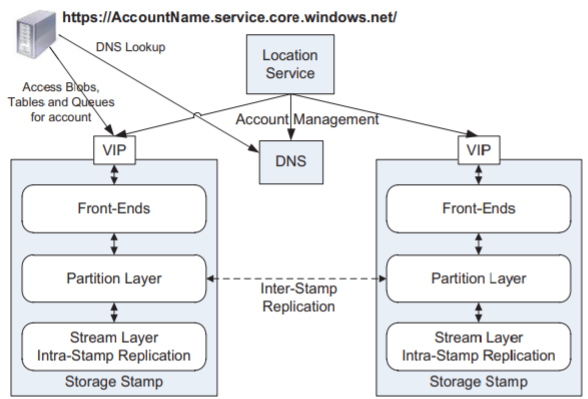
\includegraphics[scale=0.7]{images/2-was_arch.PNG}
	\caption{High-level architecture of WAS.}
	\label{fig:was_arch}
\end{figure}

\paragraph{Stream Layer (SL)}
\begin{itemize}
    \item Layer storing bits on disk, i.e. DFS within a SS.
    \item In charge of storing, distributing and replicating (intra) data across many servers within SS.
    \item \textbf{Stream:} = file = ordered list of extent pointers - managed by stream manager. Can be opened/closed/deleted/renamed/read/appended to/concatenated by PL.
    \item Extent: sequence of append blocks (up to 1GB in total). Unit of replication - typically 3 times.
    \item Block: up to $N$ bytes (typically 4MB). Minimum data unit to read and append (writes are append-only). Accessed by giving offsets (random read of stream possible).
    \item PL keeps track of object to stream / extent / block mappings.
\end{itemize}

\paragraph{Partition Layer (PL)}
\begin{itemize}
    \item Data on SL is accessed through PL.
    \item Manages and processes higher level data abstractions (blob, table, queue) and ObjectNames. Stores and caches object data on top of SL.
    \item Provides transaction ordering and strong consistency for objects.
    \item Each partition (PartitionName) is served by a different partition server.
\end{itemize}


\paragraph{Design Choices / Lessons Learned}
\begin{itemize}
    \item \textbf{Separate Storage and Compute:} Easier to scale both components independently. Layer of isolation in between in multi-user scenario. Each component does its own load balancing. Needs high bandwidth between the two.
    \item \textbf{Range Partition (Index) instead of Hashing:} Better locality and isolation for each object.
    \item \textbf{Append-Only System:} Simplifies replication protocol and handling of failure scenarios. Allows snapshots. Issue diagnosis easier. Needs good garbage collection (extra I/O).
\end{itemize}

\paragraph{Blob}
Binary large object. Collection of binary data stored as a single entity in a DBMS - usually very large ones (multimedia objects).

\paragraph{S3 vs. Azure}
See Figure \ref{fig:s3azure}.

\begin{figure}[h]
	\centering
	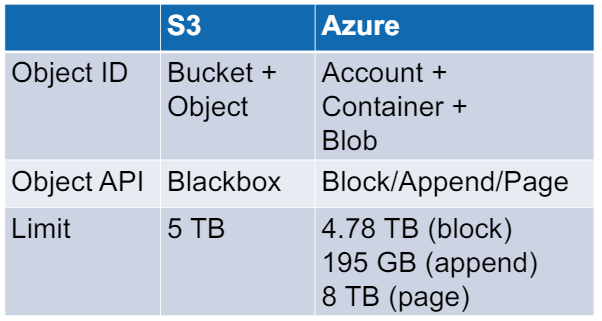
\includegraphics[scale=0.5]{images/2-s3vsazure.PNG}
	\caption{S3 vs. Azure.}
	\label{fig:s3azure}
\end{figure}



\subsection{Key-Value Store}

\paragraph{Object Store vs. Key-Value Store}
\begin{itemize}
    \item In an object store, the latency is much larger than in a typical DB (100-300ms vs. 1-9ms).
    \item Similar to object storage: store unstructured data (value) that is addressed and located with a key.
    \item In KVS, the object is much smaller than in OS (5TB vs. 400KB in Dynamo).
    \item KVS do not have metadata but keys can have variable length.
    \item Simple API: get(key) and put(key, value) (delete is just a put of nothing).
    \item KVS are very simple with little features and eventual consistency (needs conflict resolution). This allows for better performance (high availability) and scalability compared to a normal RDBMS.
    \item The most efficient data structure to query a KVS is an associative array aka. a map (single machine: tree / hash map, dis. machine: Dynamo).
\end{itemize}

%TODO more on differences?

%TODO map data structure

See reading assignment "Dynamo: Amazon's Highly Available Key-Value Store". The following is a brief summary of the paper. Many details are left out.

\paragraph{Introduction}
\begin{itemize}
    \item Always-on experience - sacrifice consistency under certain failure scenarios (CAP theorem).
    \item Eventual consistency: object versioning and application-assisted conflict resolution (quorum-like technique). All updates reach all updates eventually.
    \item Partition and replicate data using consistent hashing.
    \item Gossip-based distributed failure detection and membership protocol.
    \item Decentralized.
    \item Simple key/value interface.
    \item See summary of techniques in Figure \ref{fig:dynamo}.
\end{itemize}

\begin{figure}[h]
	\centering
	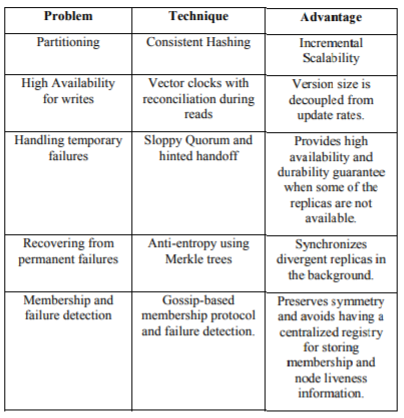
\includegraphics[scale=0.8]{images/2-dynamo.PNG}
	\caption{Techniques used in Dynamo.}
	\label{fig:dynamo}
\end{figure}

\paragraph{System Assumptions and Requirements}
\begin{itemize}
    \item Data stored as blobs, identified by unique keys. Data is small (sub 1MB).
    \item Simple read and write operations that don't span multiple data items. 
    \item No need for relational schema.
    \item No isolation guarantee, only single key updates.
    \item Commodity hardware.
    \item Non-hostile environment (Dynamo used by Amazon's internal services).
\end{itemize}

\paragraph{Service Level Agreement (SLA)}
%TODO the percentile thing, not that important, already mentioned in S3

\paragraph{Design Considerations}
\begin{itemize}
    \item Conflict resolution - when? We can always write but if we read, we need to do CR first.
    \item Conflict resolution - who? By application since data store CR is limited (last write wins). Application can choose CR method based on data schema and goals.
    \item Incremental scalability (add/remove nodes easily - needs dynamic partitioning).
    \item Symmetry (each node has the same responsibilities).
    \item Decentralization (P2P techniques, all nodes connected with all other nodes).
    \item Heterogeneity (proportional work distribution if nodes have different amount of resources).
    \item Each node knows enough routing information for zero hop latency.
\end{itemize}

\paragraph{Background}
\begin{itemize}
    \item \textbf{P2P Systems:} Unstructured (arbitrary links, "search" query flooded to find all peers holding data). Structured (any node can efficiently route requests to other node holding requested data - reduce hops by maintaining local routing info).
    \item \textbf{DFS:} %TODO, see later section, different from KVS
\end{itemize}

\paragraph{System Architecture}
\begin{itemize}
    \item \textbf{Interface:} get(key) that gives  all object replicas and their associated contexts. put(key, context, object) that writes object with key and context. Context is used for conflict resolution (see later). Keys are hashed into 128-bit IDs to locate the storage nodes responsible for serving.
    \item \textbf{Partitioning:} Consistent hashing to spread load over all storage nodes (see below).
    \item \textbf{Replication:} Per-key coordinator node replicates its data across $N-1$ nodes (clockwise successors). Per-key preference lists keep track of which nodes are allowed to store the associated objects (more than $N$). On a put-call, data is replicated asynchronously.
    \item \textbf{Data Versioning:} Modifications are treated like new items (in a put, always define which version is being modified - context). Vector clocks are used to resolve conflicts between modifications of same item (see below).
    \item See more architecture components below.
\end{itemize}

\paragraph{Consistent Hashing}
Output range of hash function treated as ring (mod $2^n$ for wrap around). Each storage node assigned to random position on ring. Hash key of object, store in node located clockwise of its hash value. Adding and removing nodes just re-assigns (transfer) all object accordingly.

\textbf{Uniform Distribution and Heterogeneity:} Randomly distribute virtual nodes (tokens) across ring. Actual nodes are assigned one or more tokens according to their capacity. Allows for better load balancing (failure, adding/removing nodes).

%TODO image?


\paragraph{Vector Clocks}
Assume the same object is updated multiple times. See Figure \ref{fig:vclock} for an example.
\begin{itemize}
    \item Create new object - written by node A.
    \item Modify this object - write by node A.
    \item Both node B and node C modify the object last modified by A at the same time.
    \item Client wants to read object and receives both versions. Client chooses the correct version based on application-specific heuristics and orders node A to write the correct version (or a new value) of the object.
\end{itemize}

%TODO more examples, exercises with this

\begin{figure}[h]
	\centering
	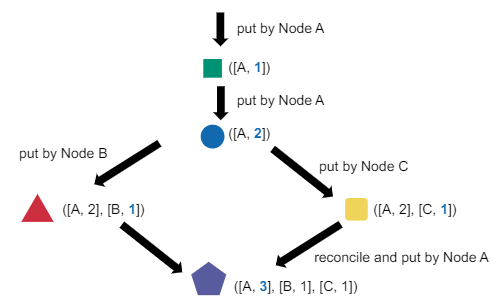
\includegraphics[scale=0.8]{images/2-vectorclock.PNG}
	\caption{Vector clock example.}
	\label{fig:vclock}
\end{figure}


\paragraph{Get and Put Execution}
\begin{itemize}
    \item \textbf{Select Node:} Either through a generic load balancer that chooses node based on some LB heuristics, that node then routes requests (to coordinator) or with a partition-aware client that routes requests directly to appropriate coordinator node. 
    \item \textbf{Coordinator Node:} Handles get/put requests, typically first of the $N$ key-specific nodes. Top $N$ healthy nodes of preference list are involved after that.
    \item \textbf{Consistency:} $R$ = min. number of nodes ACKing reads. $W$ = min. number nodes ACKing writes. Quorum-like system if $R + W > N$. Latency of operation determined by slowest node of the $R$ / $W$ nodes. Clients can tune those values! ($(N, R, W) = (3, 2, 2)$ typically).
    \item \textbf{Put:} Coordinator generates vector clock, writes new version locally, sends it to $N$ highest reachable nodes and succeeds if $W-1$ respond.
    \item \textbf{Get:} Coordinator requests all versions from $N$ highest reachable nodes, waits for $R$ responses and returns all of them to client. Client reconciles and writes back newest version.
\end{itemize}

%TODO see example in lecture

\paragraph{Failure Handling (Hinted Handoff)}
If an intended recipient node is unreachable during a write, its replica is send to next reachable node on preference list with note that it was originally intended for another node. If original node recovers, temporary node sends intended replica to it.

\paragraph{Permanent Failures}
To keep replicas synchronized (in cases where hinted replicas will not go back to intended), Merkle trees are used. Reduces amount of data that needs to be transferred when checking for inconsistencies. Each node has a Merkle tree for each key range it hosts. Two nodes exchange roots to check.

\textbf{Merkle Tree:} Leaves = hashes of values of individual keys. Parent nodes = combined hashes of children. %TODO see example

\paragraph{Membership Detection}
\begin{itemize}
    \item First time: node gets tokens, mapping kept in disk of node.
    \item Reconciliation s.t. each node has its own tokens. %TODO how?
\end{itemize}

\paragraph{Failure Detection}
If node B does not respond to node A's messages, node A considers B failed (even if it might not actually be). A periodically retries during traffic.

\paragraph{Ensuring Uniform Load Distribution}
Divide hash ring into $Q$ equally sized partitions. Each node is assigned $Q/S$ tokens where $S$ is total number of active nodes in system. %TODO ??




\subsection{Distributed File Systems}

Use OS with the KV model when dealing with a huge amount of large files and use BS with the FS model when dealing with a large amount of huge files. Now, throughput is top priority (latency is secondary).

Instead of doing random access of small parts of a file, we want to scan entire files (good for batch processing). With files, writes are append-only.

%TODO GFS?

\paragraph{Parallelism vs. Batch Processing}
Capacity has grown a lot, throughput and latency hasn't. To achieve higher throughput with lots of capacity, we can parallelize (work on different data at the same time). To achieve low latency with lots of capacity we can to batch processing (move and process large amounts of data as one unit).
%TODO more?

\paragraph{FS Logical Model}
Files are stored in a hierarchically instead of flat as in the KV model. %TODO image?

\paragraph{BS Physical Model}
A file is divided into a sequence of blocks that are exposed to the user. Files need to be broken down since they can be bigger than a single disk. In contrast, OS objects are treated as a blackbox package / collection of bits - the user does not see a further division of an object.

\paragraph{Block Size}
In a simple FS, blocks are usually 4KB. In a RDBMS, blocks are between 4KB and 32KB. In a DFS, blocks are between 64MB and 128MB.

If the size is too small, we run into latency issues (too much individual fetching). If it's too big, we run into storage issues and strain the network bandwidth. Choose the size s.t. system is dominated by throughput and not latency.

\paragraph{Hadoop}
Framework for distributed (parallel) processing of large data sets across clusters of computers using simple programming models. Each machine can do local computations and has local storage - compute close to data. Hadoop includes multiple components: HDFS, HBase, MapReduce, YARN, etc.

See reading assignment "Hadoop: The Definitive Guide". The following is a brief summary of chapter 1.

\begin{itemize}
    \item Disk storage capacities massively increased - throughput has not kept up (data reading rate).
    \item Read and write time can be reduced if we read / write from multiple disks at once = parallelism.
    \item Batch processing utilized by MapReduce - for each query, the entire dataset can be processed (see later section).
    \item MapReduce is slow and should be used for offline use. 
    \item For online access: use HBase (KVS over HDFS). Provides online read/write access of individual rows and batch operations for reading / writing data in bulk.
    \item Better processing: use YARN (cluster resource management system) - allows distributed programs to run over Hadoop cluster.
    \item Compared to RDBMS: lots of data, batch access instead of interactive and batch, write once and read many times, no ACID, schema-on-read, low integrity, linear scaling.
    \item Semi and unstructured, denormalized data.
\end{itemize}


\subsubsection{Hadoop Distributed File System (HDFS)}

See reading assignment "The Hadoop Distributed File System". The following is a brief summary of the paper. Some details and the entire "Practice at Yahoo!" section are left out. Also, see this video for an easy explanation of HDFS: \href{https://www.youtube.com/watch?v=4Gfl0WuONMY}{click.}

\paragraph{Introduction}
\begin{itemize}
    \item Store large data sets reliably and stream them at high bandwidth to user applications.
    \item Storage and computation is distributed across many servers - easy scalability.
    \item Commodity hardware.
    \item Metadata is stored in NameNodes and application data is stored in DataNodes.
    \item All servers are fully connected (master-slave architecture), communication protocols based on TCP.
    \item Reliability through replication of file content across multiple DataNodes.
    \item Single-writer, multiple-reader model (closed files can only be appended to).
\end{itemize}

\paragraph{Architecture}
Master-slave architecture with NameNode as master and multiple DataNodes as slaves. Single NameNode per cluster. See Figure \ref{fig:hdfs} and \ref{fig:hdfs_comm}.

\begin{figure}[h]
	\centering
	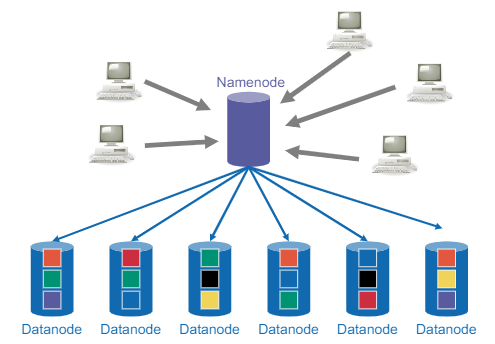
\includegraphics[scale=0.8]{images/2-hdfs.PNG}
	\caption{HDFS architecture.}
	\label{fig:hdfs}
\end{figure}

\begin{figure}[h]
	\centering
	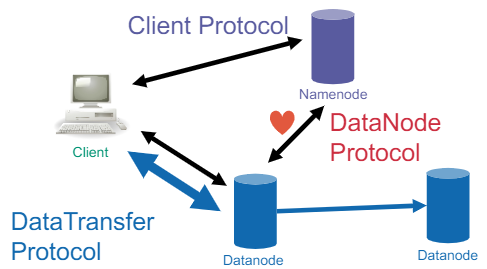
\includegraphics[scale=0.8]{images/2-hdfs_comm.PNG}
	\caption{All communication protocols in HDFS.}
	\label{fig:hdfs_comm}
\end{figure}

\paragraph{File}
File content is split into large blocks (typically 128MB, user selectable per-file) - HDFS blocks are not the same as disk blocks. Each block has a 64-bit block ID. Blocks of a file are independently replicated at multiple DataNodes (typically 3, user selectable per-file). Replica locations can change over time (not part of persistent checkpoint).

\paragraph{NameNode}
Keeps track of system-wide activity. It maintains the following in RAM: namespace tree, file to block mapping and mapping of file blocks to DataNodes (i.e. physical location of file data).

On restart, a namenode can recover the previous state by reading the namespace file (path to block ID) mapping and replaying the journal stored on its local disk (see below).

\textbf{Instructions to DN:} replicate blocks to other DNs, remove local replicas, re-register/shutdown, send block report.

\paragraph{Namespace}
Hierarchy of files and directories - represented as inodes on the NameNode (in RAM). Namespace is a tree with files as leaves, thus each file is a specific path in the tree.

A namespace gets an ID which is assigned to a HDFS instance when it is formatted. ID is persistently stored on all nodes of the cluster. Cluster belongs to one HDFS instance only!

\paragraph{inode}
Records attributes such as permissions (POSIX style), modification / access times, namespace / disk space quotas, etc.

\paragraph{Metadata}
Inode data plus list of blocks belonging to a file. Collection of all metadata = image. A persistent image is kept on the local disk of the NameNode (= checkpoint). A modification log of the image is also stored on the local disk = journal. Journal is write-ahead commit log.

\paragraph{DataNode}
Stores its HDFS blocks on local disk. Blocks can be cached in DN RAM. Each HDFS block is stored as two disk files (actual data and associated metadata). Disk files can be further divided - depends on disk, this allows access of values in the middle of a HDFS block. This also means that a 1MB file put into a 128MB HDFS block uses only 1MB of local disk space and does not fill up entire 128MB on local disk since local disk block sizes are used to store).

\textbf{Startup:} Connect to NameNode and perform handshake to verify (or assign) DataNode's namespace ID (and HDFS version). After the handshake, the DataNode registers with the NameNode with their persistently stored and never changing storage ID (assigned by a NameNode if first time).

\textbf{Block Reports:} Every hour, a DN sends a block report to NN - consists of block ID, generation stamp and block length of each block it hosts.

\textbf{Heartbeat:} Every 3 seconds, DN tells NN that it is alive and its blocks are available (and storage capacity, used capacity, nr. of current transactions). NN uses heartbeats for space allocation and load balancing mechanisms. No heartbeat: NN considers DN dead and schedules replication of its blocks to other DNs. NN never directly contacts DN, it sends instructions as replies to heartbeats.

\paragraph{Client}
User application connects to HDFS with HDFS client - read / write / delete files and create / delete directories (control). Files and directories are referenced by namespace paths. API exposes block locations to client for efficient processing.

\textbf{Read:} Ask NN for list of DN hosting replicas of blocks of file and the block IDs. Contact DN directly to retrieve blocks (closest DN first).

\textbf{Write:} Ask NN to choose list of DNs that should host replicas of first block of file. Send first block to first DN in pipeline, DN then sends it to the other DNs in prepared pipeline. After ACK, repeat for all other blocks. The replicas of the blocks of the file as individually distributed across DNs.


\paragraph{Replica Management}
\begin{itemize}
    \item NN detects if a block is under- or over-replicated with DN block reports. It then balances this with instructions.
    \item Replica 1: same node as client (or random) in rack A.
    \item Replica 2: node in different rack B.
    \item Replica 3: different node in same rack B.
    \item Replica 4 and beyond: random but if possible at most one replica per node and at most two per rack.
    \item Balancer balances disk space usage in an HDFS cluster - input threshold value (fraction in range from 0 to 1). Cluster is balanced if for each DN, its utilization (ratio of used space to total capacity) differs from utilization of whole cluster by no more than threshold value. It iteratively moves replicas from DN with high util. to DN with low util. Process is optimized by minimizing inter-rack data copying.
    \item Removing a replica: system tries not to reduce number of racks hosting replica and tries to remove it from DN with least amount of space.
\end{itemize}

%TODO examples for replica placing

\paragraph{Distance Calculation}
See Figures \ref{fig:dist1} and \ref{fig:dist2}.

\begin{figure}[h]
	\centering
	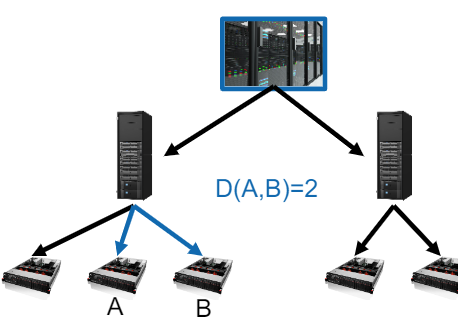
\includegraphics[scale=0.6]{images/2-dist1.PNG}
	\caption{Calculate distance in HDFS.}
	\label{fig:dist1}
\end{figure}

\begin{figure}[h]
	\centering
	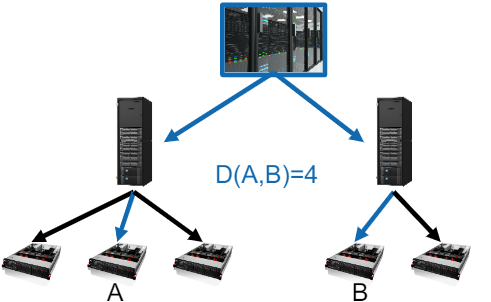
\includegraphics[scale=0.6]{images/2-dist2.PNG}
	\caption{Calculate distance in HDFS.}
	\label{fig:dist2}
\end{figure}

\paragraph{Backup}
Secondary Namenode keeps namespace image and edit log of primary NameNode, periodically merges namespace image and edit log. (Alternative: federated DFS with multiple NN responsible for partitions of namespace.(
%TODO watch lecture on backup if NN fails


%TODO using HDFS at end?
%TODO HDFS vs GFS

\paragraph{Hadoop: The Definitive Guide}
See reading assignment "Hadoop: The Definitive Guide". The following is a brief summary of chapter 3 (of points not yet mentioned above).

\begin{itemize}
    \item Huge files: hundreds of MB, GB or TB in size. Hadoop clusters store PB of data. We don't want lots of small files.
    \item Write-once, read-many-times data processing pattern. Analysis involves large proportion of / entire dataset. Time to read it (throughput) is more important than latency of reading first record.
    \item Not good for low-latency applications. We have high throughput.
    \item HDFS block is not the same as disk block!
    \item etc.
\end{itemize}
%TODO maybe more if exercises more complicated




\subsection{Syntax}

Physical representation of data on a syntax level (files). Examples include: text, CSV, XML, JSON, etc. The files we feed into a Big Data storage system are written in any of those formats.

These formats allow for data to be represented in a denormalized (non-atomic values, nestedness) and heterogeneous (rows don't all have values for all attributes) way. Such data can be queried with NoSQL systems.

For read-intensive workloads, denormalized data works well - if we avoid joins (they can be impossible). In contrast, for write-intensive workloads, we want high levels of normalization to avoid update anomalies (and else).

\paragraph{Comma Separated Values (CSV)}
A CSV file can be easily represented as a table. The first row are the attribute names and all following rows are the attribute values. Words are separated by comma (or else in other standards).

\paragraph{Structured}
A normalized table.

\paragraph{Semi-Structured}
Document can be expressed in a tree data model (XML, JSON, etc. - see later).

\paragraph{Unstructured}
A text file.

\paragraph{Well-Formedness}
A document is well-formed if it actually belongs to the language it is written in (abides to the syntax / grammar rules). Else, it is not well-formed.


\subsubsection{JSON}

See reading assignment "JSON ECMA Standard". The following is a brief summary.

\paragraph{Introduction}
\begin{itemize}
    \item JSON = text syntax, facilitates structured data interchange between programming languages. 
    \item Language-independent - used to define data interchange formats.
    \item Meaningful data interchange requires agreement between producer and consumer on semantics attached to particular use of JSON syntax (see later section).
    \item Agnostic to semantics of numbers. Numbers are simply a sequence of digits.
    \item Simple notation to express collections of name/value pairs.
    \item Support for ordered lists of values (that can also be nested).
    \item No support for cyclic graphs.
    \item Not for applications requiring binary data.
\end{itemize}

\paragraph{Text}
Sequence of tokens. Six structural tokens (square brackets, curly brackets, colon and comma), strings, numbers and three literal name tokens (true, false, null). Whitespace is allowed everywhere besides inside tokens (except inside strings).

\paragraph{Values}
\begin{itemize}
    \item \textbf{Object:} Curly bracket tokens surrounding zero or more name/value pairs. Names are always string and followed by single colon. Commas separate value from next name. Names don't have to be unique (but really should be...) and the name/value ordering doesn't matter. %TODO well formed if same name?
    \item \textbf{Array:} Square bracket tokens surrounding zero or more values separated by commas. Ordering doesn't matter.
    \item \textbf{Number:} Any sequence of decimal digits, leading minus okay, decimal point okay, exponent okay. Inf and NaN not permitted.
    \item \textbf{String:} Sequence of unicode code points wrapped by quotation marks. Some code points must be escaped (see below). Any code point can also be written in hex representation. %TODO examples \usequence
    \item \textbf{true / false / null}
\end{itemize}

%TODO examples for well and not well formed

\paragraph{String Escapes}
Reverse solidus followed by: quotation marks, reverse solidus, solidus, b for backspace, f for form feed, n for line feed, r for carriage return, t for tabulation character.
%TODO what are the last ones (unicode)


\paragraph{Some Examples}
See JSON examples below (taken from the slides).

\begin{lstlisting}[language=json,firstnumber=1]
{
    "target": "Italian",
    "sample": "af45858ejdgi02i3n4j",
    "choices": ["Chinese", true, {"foo": false}, null, 3.12],
    "bar": true,
    "object": {"School": "ETH"},
    "Q": null
    "Exponent": -1.23E+5,
    "unicode": "foo\nbar\u005f"
}
\end{lstlisting}



\subsubsection{XML}

See reading assignment "XML in a Nutshell". The following is a brief summary of chapters 1, 2, 4.1, 4.2 and 16.

\paragraph{Introduction}
\begin{itemize}
    \item Generic syntax to mark up data with simple, human-readable tags.
    \item Provides standard format for documents that is flexible enough to be customized for various domains.
    \item Basically the same as above.
    \item XML application: tag set defined by individuals / companies if their application only wants to use a subset of XML tags.
    \item Documents can be associated with an XML schema to check for validity (does the document fit a given mold). See later section.
    \item XML document contains text, never binary data. XML documents are simply text files with a special structure (just like with JSON) read by XML parsers.
\end{itemize}

\paragraph{Fundamentals}
\begin{itemize}
    \item \textbf{Element:} Start-tag, content, end-tag. The tags name the element. Elements can contain more elements (surrounded by content). E.g.  $<$person$>$ Alan Turing $<$/person$>$ - this element is called "person".
    \item \textbf{Empty Element:} $<$person$><$/person$>$ is the same as $<$person/$>$.
    \item XML is case-sensitive.
    \item XML document is a tree: nested tags with content. Only one root = document element. Each child has only one parent and a parent can have several children. XML doc must start with an element. See example below.
    \item \textbf{Attributes:} Elements can have attributes = name-value pairs, attached to the start-tag. E.g. $<$person born="1912-06-23" died="1954-06-07"$>$ Alan Turing $<$/person$>$ (single instead of double quotes is okay).
    \item Convention: data is content and metadata / additional info for data is attribute.
    \item \textbf{Names (element / attribute):} May only contain characters defined in Unicode 3.0 and later, no length limit, can contain A-Z, a-z, 0-9, non-English letters, dot, minus, underscore. Don't start with "xml" (reserved). Don't start with a number. %TODO correct?
    \item \textbf{References:} escape $<$ character with "\&lt;" tag (entity reference), "\&\#60;" (numeric character reference) or "\&\#x3C;" (hex. num. char. reference). Escape \& with "\&amp;" or "\&\#38;". There is also "\&gt;" for $>$, "\&quot;" for " and "\&apos;" for '. Sequence "]]$>$" must be written "]]\&gt;". %TODO nicer format
    \item \textbf{CDATA Sections:} If a text includes many escape characters, put text in a CDATA section: $<$![CDATA[ \&$<>$" hello, $<<<$]]$>$ - everything in [] is treated as raw character data.
    \item \textbf{Comment:} $<$!-- example--$>$, double hyphen never inside comment text. Comments can appear anywhere. Don't use additional hyphen to close (---$>$).
    \item \textbf{Processing Instructions:} Alternative way to pass info (in any syntax, can be code) to particular application reading the XML document. Begins with $<$? and ends with ?$>$. Can appear anywhere. Don't put XML and variations of that into it. %TODO more?
    \item \textbf{XML Declaration:} Looks the same as processing instruction. Not necessary but if included must be very first thing. Always use version 1.0. Default encoding is UTF-8. Encoding specified by metadata wins if in conflict with declaration. Standalone: if not standalone, application might need to read external DTD to determine proper values for parts of doc - default is no.
\end{itemize}

%todo allowed chars in names



\begin{lstlisting}[language=XML]
<?xml version="1.0" encoding="ASCII" standalone="yes"?>
<!-- example XML decl. above -->

<person>
  <name>
    <first_name>Alan</first_name>
    <last_name>Turing</last_name>
  </name>
  <profession>computer scientist</profession>
  <profession>mathematician</profession>
  <profession>cryptographer</profession>
</person>

<!-- same as above (with attributes): -->

<person>
  <name first="Alan" last="Turing"/>
  <profession value="computer scientist"/>
  <profession value="mathematician"/>
  <profession value="cryptographer"/>
</person>
\end{lstlisting}

\begin{figure}[h]
	\centering
	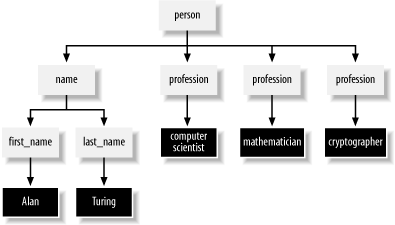
\includegraphics[scale=0.6]{images/2-xmltree.png}
	\caption{The person XML as a tree.}
	\label{fig:xmltree}
\end{figure}

\paragraph{Checking for Well-Formedness}
\begin{itemize}
    \item Every start-tag must have a matching end-tag.
    \item Elements may nest but may not overlap.
    \item There must be exactly one root element.
    \item Attribute values must be quoted.
    \item An element may not have two attributes with the same name.
    \item Comments and processing instructions may not appear inside tags.
    \item No unescaped $<$ or \& signs may occur in the character data of an element or attribute.
    \item No whitespace in element tag.
    \item No "lower case" quotation marks.
\end{itemize} %TODO see examples

%TODO more examples, what can content be



%TODO doctype?? see slides (or chapter 3)



\paragraph{Namespaces}
Distinguish between elements / attributes from different vocabularies with different meaning that happen to have the same name and group all related elements / attributes from a single XML application together (easy to recognize for software). E.g. a join of two datasets with different meaning (networks vs. CRM) - two elements might have the name "client".

\begin{itemize}
    \item With a namespace, a local name turns into an expanded name.
    \item Namespace implementation: attach a prefix to each element and attribute. Each prefix is mapped to a URI. Same namespace if element / attribute has same prefix.
    \item URI / IRI doesn't actually have to map to a resolved webpage.
    \item Qualified name (Qname / Raw Name): prefix:localname and namespace URI.
    \item Localname identifies element within the namespace.
    \item If the prefix is not specified, we are simply in the default namespace - use rarely. Prefixed elements are in their namespace but non-prefixes children in default namespace. Unprefixed attributes are never in any namespace even if they're in scope.
    \item If the local name and namespace is the same but the prefixes differ, we still have the same Qname. Same attribute name and namespace but different prefix is not well-formed.
    \item To make it tidier, namespace bindings can be put into root element.
    \item Backward compatibility: parser that doesn't know any namespaces will have no problem reading document with.
\end{itemize}

\begin{lstlisting}[language=XML]
<prefix:localname xmlns:prefix="http://example.com/prefix">

<!-- scope of prefix namespace binding -->

</prefix:localname>
\end{lstlisting}

\begin{lstlisting}[language=XML]
<!-- example of default namespace: -->

<math xmlns="http://www.w3.org/1998/Math/MathML">

</math xmlns="http://www.w3.org/1998/Math/MathML">
\end{lstlisting}

\begin{lstlisting}[language=XML]
<!-- tidy example: -->

<?xml version "1.0"?>

<prefix1:foo
    xmlns:prefix1="http://example.com/prefix1"
    xmlns:prefix2="http://example.com/prefix2">
    
    <prefix1:some_name>
        "Something"
    </prefix1:some_name>
    
    <prefix2:other_name prefix2:attr="value">
        "Hello!"
    </prefix2:other_name>
    
</prefix1:foo>
\end{lstlisting}

%TODO above example: prefix2 repeat if prefix also for attribute? or remove prefix2 from element tag???????



%TODO oxygen (free download eth)
%TODO YAML?























\subsection{Exercises}

\subsubsection{Object and Key-Value Stores}

\subsubsection{HDFS}

\subsubsection{XML}